\documentclass[10pt]{beamer}

% Set beamer-theme
\usetheme[progressbar=frametitle]{metropolis}
\usepackage{appendixnumberbeamer}

\usepackage{algorithm, algorithmic}
\renewcommand{\algorithmiccomment}[1]{// #1}

% Display more advanced math
\usepackage{amsmath}
% Command to display variable names in upright font
\newcommand*{\var}[1]{\operatorname{#1}}

% Display values with SI units beatifully
\usepackage{siunitx}
\sisetup{group-minimum-digits = 3}

% Make references take you not to the caption but the whole table/image
\usepackage{caption}

% Allow long tables to span multiple mages
\usepackage{longtable}

% Easily draw square arrays
\usepackage[thinlines]{easytable}

% Draw a graph in LaTeX
\usepackage{tikz}
\usetikzlibrary{arrows}

% Add images
\usepackage{graphicx}
\graphicspath{ {img/} }

% Allow font specifications
\usepackage{fontspec}
% Allow multiple languages in the text
\usepackage{polyglossia}
\setdefaultlanguage{greek}
\setotherlanguage{english}
\setsansfont[
    Extension      = .ttf,
    UprightFont    = *,
    ItalicFont     = *i,
    BoldFont       = *b,
    BoldItalicFont = *z,
    Ligatures      = TeX,
    Path           = fonts/
]{cambria}
\setmonofont{Courier}
\newfontfamily{\greekfont}[
    Extension      = .ttf,
    UprightFont    = *,
    ItalicFont     = *i,
    BoldFont       = *b,
    BoldItalicFont = *z,
    Ligatures      = TeX,
    Path           = fonts/
]{cambria}
\newfontfamily{\greekfonttt}{Courier}
\newfontface{\TVSp}{DejaVu Sans Mono}
\def\textvisiblespace{{\TVSp\char"2423}}

\gappto\captionsgreek{
    \def\equationautorefname{Εξίσωση}
    \def\footnoteautorefname{υποσημείωση}
    \def\itemautorefname{στοιχείο}
    \def\figureautorefname{Σχήμα}
    \def\tableautorefname{Πίνακα}
    \def\partautorefname{Μέρος}
    \def\appendixautorefname{Παράρτημα}
    \def\chapterautorefname{Κεφάλαιο}
    \def\sectionautorefname{Eνότητα}
    \def\subsectionautorefname{Υποενότητα}
    \def\subsubsectionautorefname{Υπο-υποενότητα}
    \def\paragraphautorefname{Παράγραφο}
    \def\subparagraphautorefname{Υποπαράγραφο}
    \def\FancyVerbLineautorefname{γραμμή}
    \def\theoremautorefname{Θεώρημα}
    \def\pageautorefname{σελίδα}
    \def\lstlistingname{Κώδικας}
    \def\lstlistingautorefname{Κώδικας}
}

% Recomended for correct quotes
\usepackage{csquotes}

\newenvironment{alltt}{\ttfamily}{\rmfamily}

%Information to be included in the title page:
\title[Ασφάλεια Συστημάτων Υπολογιστών]{
    Ανεύρεση Κωδικού με Χρήση Μαρκοβιανών Αλυσίδων \\[10pt]
}

\subtitle{
    Ασφάλεια Συστημάτων Υπολογιστών \\
    Γεώργιος Δροσάτος
}

\author{
    Αναστασιάδου Μαγδαλινή \and Γκαντίδης Χρήστος
}

\institute[Δ.Π.Θ.]{
Τμήμα Ηλεκτρολόγων Μηχανικών και Μηχανικών Υπολογιστών\\
Δημοκρίτειο Πανεπιστήμιο Θράκης
}
\date{Ιανουάριος 2018}

\begin{document}

% Title page
\maketitle

% Contents
\begin{frame}{Περιεχόμενα}
    \setbeamertemplate{section in toc}[sections numbered]
    \tableofcontents[hideallsubsections]
\end{frame}

% Markov chains
\section{Περίληψη Μαρκοβιανών Αλυσίδων}
    \begin{frame}{Μαρκοβιανές αλυσίδες}
        \begin{block}{Ορισμός}
            Οι Μαρκοβιανές αλυσίδες, είναι μαθηματικές κατασκευές οι οποίες περιγράφουν την μετάβαση ενός συστήματος από μια κατάσταση σε όλες τις υπόλοιπες δυνατές καταστάσεις του συστήματος.
        \end{block}
        \pause
        \begin{block}{Παράδειγμα}
            Πώς θα μπορούσαμε να αναπαραστήσουμε τις μεταβάσεις ενός συστήματος το οποίο περιγράφει
            τον καιρό μιας περιοχής, θεωρώντας 2 δυνατές καταστάσεις \{\textit{λιακάδα}, \textit{συννεφιά}\};
        \end{block}
    \end{frame}
\begin{frame}{Μαρκοβιανές αλυσίδες}
    Για 2 δυνατές καταστάσεις, υπάρχουν 4 δυνατές μεταβάσεις, καθώς από κάθε κατάσταση υπάρχει η πιθανότητα να μεταβούμε στην άλλη ή να παραμείνουμε στην ίδια. Γενικά για κάθε $n$ καταστάσεις υπάρχουν $n^2$ δυνατές μεταβάσεις.

    \begin{figure}[h]
        \centering
        \begin{tikzpicture}
        [nstyle/.style={circle, draw=blue!50, fill=blue!20, thick, inner sep=0em, minimum size=6em},
        vstyle/.style={circle, fill=white},
        dstyle/.style={->, very thick}]

        \node[vstyle] (sunny1)  at (0,0) {0.7};
        \node[nstyle] (sunny)   at (2,0) {λιακάδα};
        \node[nstyle] (cloudy)   at (6,0) {συννεφιά};
        \node[vstyle] (cloudy1)  at (8,0) {0.6};

        \draw[dstyle] (sunny) to[bend left=45] node[circle,fill=white]{0.3} (cloudy);
        \draw[dstyle] (cloudy) to[bend left=45] node[circle,fill=white]{0.4} (sunny);
        \draw[very thick] (sunny) to[in=90, out=135] (sunny1);
        \draw[dstyle] (sunny1) to[in=225, out=270] (sunny);
        \draw[very thick] (cloudy) to[in=270, out=315] (cloudy1);
        \draw[dstyle] (cloudy1) to[in=45, out=90] (cloudy);
        \end{tikzpicture}
    \end{figure}
\end{frame}

\begin{frame}{Μαρκοβιανές αλυσίδες}
    Επειδή για μεγαλύτερα $n$ οι αναπαραστάσεις με μορφή γράφου αρχίζουν να γίνονται χαοτικές, προτιμούμε την αναπαράσταση των Μαρκοβιανών αλυσίδων με μορφή πίνακα.
    \begin{table}[h]
        \centering
        \begin{TAB}(c){c|c|c|}{c|c|c|}
            & λιακάδα   & συννεφιά  \\
            λιακάδα     & $0.7$     & $0.3$     \\
            συννεφιά    & $0.4$     & $0.6$     \\
        \end{TAB}
    \end{table}
\end{frame}

% Hash functions
\section{Κατακερματισμός Κωδικών}
\begin{frame}{Hash Functions}
    \begin{block}{Ορισμός}
        Οι \textit{Συναρτήσεις Κατακερματισμού (hash functions)}, είναι συναρτήσεις οι οποίες δέχονται ως είσοδο δεδομένα οποιουδήποτε μεγέθους, και τα αντιστοιχίζουν ντετερμινιστικά σε κάποια άλλα δεδομένα σταθερού μεγέθους.
    \end{block}
    \pause
    \begin{block}{Χρήση}
        Αποθήκευση κωδικών των χρηστών μιας σελίδας, στην βάση δεδομένων, με στόχο την προστασία των προσωπικών δεδομένων τους.
    \end{block}
\end{frame}

\begin{frame}{Hash Functions}
    \begin{block}{Κωδικοί με το MD5 hash τους}
        \begin{table}[h]
            \centering
            \begin{alltt}
                \begin{TAB}(r){l|r|}{c|ccc|}
                    \rmfamily{κωδικός}     & \rmfamily{MD5 hash} \\
                    apple                  & 1f3870be274f6c49b3e31a0c6728957f \\
                    Apple                  & 9f6290f4436e5a2351f12e03b6433c3c \\
                    apple\textvisiblespace & e307c4bc0265c934316dbd59f86336fd \\
                \end{TAB}
            \end{alltt}
        \end{table}
    \end{block}
\end{frame}

\begin{frame}{Hash Functions}
    Για να βρούμε ποιος κωδικός απλού κειμένου αντιστοιχεί στον κωδικό κατακερματισμού πρέπει:
    \pause

    \begin{itemize}
        \item[ή] Να ξέρουμε εξαρχής τον κωδικό απλού κειμένου.
        \pause
        \item[ή] Nα δοκιμάσουμε διάφορους κωδικούς απλού κειμένου ως εισόδους της συνάρτησης μέχρι να βρούμε την έξοδο που είναι ίδια με τον κατακερματισμένο κωδικό.
    \end{itemize}
\end{frame}

% Guessing methods
\section{Μέθοδοι Ανεύρεσης}
\begin{frame}{Brute force}
    \begin{block}{Ορισμός}
        Δοκιμάζουμε όλους τους πιθανούς συνδυασμούς των χαρακτήρων που ανήκουν στο \textit{πεδίο χαρακτήρων (character space)}, συνήθως κατά αύξουσα σειρά.
    \end{block}
    \pause
    \begin{block}{Παράδειγμα}
        Έστω \textit{character space = (a--z)} και ότι θέλουμε να δοκιμάσουμε όλους τους κωδικούς με μήκος τρεις χαρακτήρες, τότε οι κωδικοί θα δοκιμαστούν με την ακόλουθη σειρά.
        \begin{table}[h]
            \centering
            \begin{alltt}
                \begin{tabular}{ccccccc}
                    aaa & aba & $\cdots$ & baa & bba & $\cdots$ & zza \\
                    aab & abb & $\cdots$ & bab & bbb & $\cdots$ & zzb \\
                    aac & abc & $\cdots$ & bac & bbc & $\cdots$ & zzc \\
                    $\vdots$ & $\vdots$ & $\ddots$ & $\vdots$ & $\vdots$ & $\ddots$ & $\vdots$ \\
                    aaz & abz & $\cdots$ & baz & bbz & $\cdots$ & zzz \\
                \end{tabular}
            \end{alltt}
        \end{table}
    \end{block}
\end{frame}

\begin{frame}{Dictionary attack}
    \begin{block}{Ορισμός}
        Η μέθοδος λεξικού (dictionary attack) βασίζεται στην δοκιμή λέξεων από μια υπάρχουσα λίστα. Περιορίζεται μόνο σε συνηθισμένες ακολουθίες χαρακτήρων που είναι εύκολο να απομνημονευθούν.
    \end{block}
    \pause
    \begin{block}{Παράδειγμα}
        Το πλήθος των λέξεων στο Oxford English Dictionary είναι περίπου \SI{600000}, θεωρώντας ότι ο μέσος άνθρωπος χρησιμοποιεί, από \SI{10000} εώς \SI{40000} από αυτές, με έναν ρυθμό δοκιμής \SI{5000000} κωδικών το δευτερόλεπτο, θα απαιτούνταν γύρω στα \SI{8}{ms} για να δοκιμαστούν όλες οι λέξεις!
    \end{block}
\end{frame}

\begin{frame}{Markov Chains}
    \begin{block}{Ορισμός}
        Με την χρήση των Μαρκοβιανών αλυσίδων, μπορούμε να βελτιώσουμε την μέθοδο ωμής βίας. Στις λέξεις της φυσικής γλώσσας, η συχνότητα και η ακολουθία των γραμμάτων δεν είναι ισοπίθανη.
    \end{block}
    \pause
    \begin{block}{Παράδειγμα}
        Στην Αγγλική γλώσσα, περισσότερες λέξεις ξεκινάνε με τον χαρακτήρα \texttt{'c'} παρά με τον χαρακτήρα \texttt{'b'}. Επίσης, υπάρχουν περισσότερες λέξεις, στις οποίες ο χαρακτήρας \texttt{'a'} ακολουθείται από τον χαρακτήρα \texttt{'b'}, παρά από τον χαρακτήρα \texttt{'a'}.
    \end{block}
\end{frame}

\begin{frame}{Σύγκριση μεθόδων}
    \begin{table}
        \begin{tabular}{l|c|c|c}
                        & Brute Force           & Dictionary            & Markov Chains \\\hline
        Πολυπλοκότητα   & $\mathcal{O}(s^n)$    & $\mathcal{O}(l)$      & $\mathcal{O}(t^n)$ \\
        \end{tabular}
    \end{table}

    \begin{description}
        \item[$n$] μήκος του κωδικού απλού κειμένου
        \item[$s$] πληθικότητα του πεδίου χαρακτήρων
        \item[$l$] πλήθος λέξεων στο λεξικό
        \item[$t$] πληθικότητα του πεδίου χαρακτήρων $t \le s$
    \end{description}
\end{frame}

% Implementation of Markov Chains
\section{Υλοποίηση Μεθόδου Μαρκοβιανών Αλυσίδων}
\begin{frame}{Παραγωγή Μαρκοβιανών Πινάκων}
    \begin{block}{Στόχος}
        \begin{itemize}
            \item Να δημιουργήσουμε ένα Μαρκοβιανό πίνακα για κάθε θέση του κωδικού (per position Markov table).
            \item Να χρησιμοποιήσουμε τους πίνακες για να παράγουμε πραγματικούς κωδικούς!
        \end{itemize}
    \end{block}
    \pause
    \begin{block}{Χαρακτηριστικά υλοποίησης}
        \begin{itemize}
            \item Οι πίνακες μπορούν να παραχθούν από οποιαδήποτε λίστα κωδικών απλού κειμένου \textit{(wordlist)}.
            \item Οι κωδικοί έχουν μήκος μέχρι 10 χαρακτήρες.
            \item Το πεδίο χαρακτήρων είναι το πλήρες διάστημα εκτυπώσιμων χαρακτήρων του πίνακα ASCII (κωδικοί 32--126), με πληθικότητα 95.
        \end{itemize}
    \end{block}
\end{frame}

\begin{frame}{Χαρακτηριστικά υλοποίησης}
    \begin{block}{Πόσους πίνακες θα χρειαστούμε;}
        Αφού από κάθε μια κατάσταση, μπορούμε να πάμε σε οποιαδήποτε κατάσταση, δημιουργούμε έναν πίνακα με διαστάσεις 95$\times$95 για κάθε θέση, δηλαδή 10 στο πλήθος.
    \end{block}
    \pause
    \begin{block}{Πώς θα αναπαραστήσουμε τους πίνακες;}
        Υπό την μορφή ενός τρισδιάστατου πίνακα, με μήκος 1\textsuperscript{ης} διάστασης το μέγιστο μήκος κωδικού και μήκος 2\textsuperscript{ης} και 3\textsuperscript{ης} διάστασης την πληθικότητα του πεδίου χαρακτήρων.
    \end{block}
\end{frame}

\begin{frame}{Αλγόριθμος παραγωγής Μαρκοβιανών Πινάκων}
    \begin{algorithm}[H]
        \small
        \caption{Generate Markov Tables}
        \label{alg:gen_markov_tables}
        \algsetup{indent=2em}
        \begin{algorithmic}[1]
            \STATE{} \COMMENT{Initialize all frequencies to 0}
            \FOR{$m=0$ to $9$}
                \FOR{$i=0$ to $94$}
                    \FOR{$j=0$ to $94$}
                        \STATE{$markov[m][i][j] = 0$}
                    \ENDFOR
                \ENDFOR
            \ENDFOR

            \STATE{} \COMMENT{Compute Frequencies}
            \FORALL{$words$ in $dictionary$}
                \STATE{$markov[0][0][word[0]] \mathrel{{+}{=}} 1$}
                \FOR{$c=1$ to $length(word)$}
                    \STATE{$markov[c][word[c-1]][word[c]] \mathrel{{+}{=}} 1$}
                \ENDFOR
            \ENDFOR
        \end{algorithmic}
    \end{algorithm}
\end{frame}

\begin{frame}{Παράδειγμα}
    \begin{block}{Υποθέσεις}
        \begin{itemize}
            \item Το πεδίο χαρακτήρων είναι το \{a, b, c, d, e\}
            \item Το μέγιστο μήκος κωδικού είναι 4
            \item Η λίστα με τους κωδικούς είναι η ακόλουθη
            \begin{table}
                \begin{tabular}{ll}
                    ace & bee \\
                    add & cab \\
                    bad & dad \\
                    bed & dead \\
                \end{tabular}
            \end{table}
        \end{itemize}
    \end{block}
\end{frame}

\begin{frame}{Παράδειγμα}
    \only<1> {
        \begin{block}{Βήμα 0: Αρχικοποίηση}
            \begin{TAB}(c){cccc}{cc}
                \begin{TAB}(e)[3pt]{|c:c:c:c:c|}{|c:c:c:c:c|}
                    0 & 0 & 0 & 0 & 0 \\
                    0 & 0 & 0 & 0 & 0 \\
                    0 & 0 & 0 & 0 & 0 \\
                    0 & 0 & 0 & 0 & 0 \\
                    0 & 0 & 0 & 0 & 0 \\
                \end{TAB}
                &
                \begin{TAB}(e)[3pt]{|c:c:c:c:c|}{|c:c:c:c:c|}
                    0 & 0 & 0 & 0 & 0 \\
                    0 & 0 & 0 & 0 & 0 \\
                    0 & 0 & 0 & 0 & 0 \\
                    0 & 0 & 0 & 0 & 0 \\
                    0 & 0 & 0 & 0 & 0 \\
                \end{TAB}
                &
                \begin{TAB}(e)[3pt]{|c:c:c:c:c|}{|c:c:c:c:c|}
                    0 & 0 & 0 & 0 & 0 \\
                    0 & 0 & 0 & 0 & 0 \\
                    0 & 0 & 0 & 0 & 0 \\
                    0 & 0 & 0 & 0 & 0 \\
                    0 & 0 & 0 & 0 & 0 \\
                \end{TAB}
                &
                \begin{TAB}(e)[3pt]{|c:c:c:c:c|}{|c:c:c:c:c|}
                    0 & 0 & 0 & 0 & 0 \\
                    0 & 0 & 0 & 0 & 0 \\
                    0 & 0 & 0 & 0 & 0 \\
                    0 & 0 & 0 & 0 & 0 \\
                    0 & 0 & 0 & 0 & 0 \\
                \end{TAB}

                \\

                markov[$0$] & markov[$1$] & markov[$2$] & markov[$3$]
            \end{TAB}
        \end{block}
    }

    \only<2> {
        \begin{block}{Βήμα 1: ace}
            \begin{TAB}(c){cccc}{cc}
                \begin{TAB}(e)[3pt]{|c:c:c:c:c|}{|c:c:c:c:c|}
                    \textcolor{red}{1} & 0 & 0 & 0 & 0 \\
                    0 & 0 & 0 & 0 & 0 \\
                    0 & 0 & 0 & 0 & 0 \\
                    0 & 0 & 0 & 0 & 0 \\
                    0 & 0 & 0 & 0 & 0 \\
                \end{TAB}
                &
                \begin{TAB}(e)[3pt]{|c:c:c:c:c|}{|c:c:c:c:c|}
                    0 & 0 & \textcolor{red}{1} & 0 & 0 \\
                    0 & 0 & 0 & 0 & 0 \\
                    0 & 0 & 0 & 0 & 0 \\
                    0 & 0 & 0 & 0 & 0 \\
                    0 & 0 & 0 & 0 & 0 \\
                \end{TAB}
                &
                \begin{TAB}(e)[3pt]{|c:c:c:c:c|}{|c:c:c:c:c|}
                    0 & 0 & 0 & 0 & 0 \\
                    0 & 0 & 0 & 0 & 0 \\
                    0 & 0 & 0 & 0 & \textcolor{red}{1} \\
                    0 & 0 & 0 & 0 & 0 \\
                    0 & 0 & 0 & 0 & 0 \\
                \end{TAB}
                &
                \begin{TAB}(e)[3pt]{|c:c:c:c:c|}{|c:c:c:c:c|}
                    0 & 0 & 0 & 0 & 0 \\
                    0 & 0 & 0 & 0 & 0 \\
                    0 & 0 & 0 & 0 & 0 \\
                    0 & 0 & 0 & 0 & 0 \\
                    0 & 0 & 0 & 0 & 0 \\
                \end{TAB}

                \\

                markov[$0$] & markov[$1$] & markov[$2$] & markov[$3$]
            \end{TAB}
        \end{block}
    }

    \only<3> {
        \begin{block}{Βήμα 2: add}
            \begin{TAB}(c){cccc}{cc}
                \begin{TAB}(e)[3pt]{|c:c:c:c:c|}{|c:c:c:c:c|}
                    \textcolor{red}{2} & 0 & 0 & 0 & 0 \\
                    0 & 0 & 0 & 0 & 0 \\
                    0 & 0 & 0 & 0 & 0 \\
                    0 & 0 & 0 & 0 & 0 \\
                    0 & 0 & 0 & 0 & 0 \\
                \end{TAB}
                &
                \begin{TAB}(e)[3pt]{|c:c:c:c:c|}{|c:c:c:c:c|}
                    0 & 0 & 1 & \textcolor{red}{1} & 0 \\
                    0 & 0 & 0 & 0 & 0 \\
                    0 & 0 & 0 & 0 & 0 \\
                    0 & 0 & 0 & 0 & 0 \\
                    0 & 0 & 0 & 0 & 0 \\
                \end{TAB}
                &
                \begin{TAB}(e)[3pt]{|c:c:c:c:c|}{|c:c:c:c:c|}
                    0 & 0 & 0 & 0 & 0 \\
                    0 & 0 & 0 & 0 & 0 \\
                    0 & 0 & 0 & 0 & 1 \\
                    0 & 0 & 0 & \textcolor{red}{1} & 0 \\
                    0 & 0 & 0 & 0 & 0 \\
                \end{TAB}
                &
                \begin{TAB}(e)[3pt]{|c:c:c:c:c|}{|c:c:c:c:c|}
                    0 & 0 & 0 & 0 & 0 \\
                    0 & 0 & 0 & 0 & 0 \\
                    0 & 0 & 0 & 0 & 0 \\
                    0 & 0 & 0 & 0 & 0 \\
                    0 & 0 & 0 & 0 & 0 \\
                \end{TAB}

                \\

                markov[$0$] & markov[$1$] & markov[$2$] & markov[$3$]
            \end{TAB}
        \end{block}
    }

    \only<4> {
        \begin{block}{Βήμα 3: bad}
            \begin{TAB}(c){cccc}{cc}
                \begin{TAB}(e)[3pt]{|c:c:c:c:c|}{|c:c:c:c:c|}
                    2 & \textcolor{red}{1} & 0 & 0 & 0 \\
                    0 & 0 & 0 & 0 & 0 \\
                    0 & 0 & 0 & 0 & 0 \\
                    0 & 0 & 0 & 0 & 0 \\
                    0 & 0 & 0 & 0 & 0 \\
                \end{TAB}
                &
                \begin{TAB}(e)[3pt]{|c:c:c:c:c|}{|c:c:c:c:c|}
                    0 & 0 & 1 & 1 & 0 \\
                    \textcolor{red}{1} & 0 & 0 & 0 & 0 \\
                    0 & 0 & 0 & 0 & 0 \\
                    0 & 0 & 0 & 0 & 0 \\
                    0 & 0 & 0 & 0 & 0 \\
                \end{TAB}
                &
                \begin{TAB}(e)[3pt]{|c:c:c:c:c|}{|c:c:c:c:c|}
                    0 & 0 & 0 & \textcolor{red}{1} & 0 \\
                    0 & 0 & 0 & 0 & 0 \\
                    0 & 0 & 0 & 0 & 1 \\
                    0 & 0 & 0 & 1 & 0 \\
                    0 & 0 & 0 & 0 & 0 \\
                \end{TAB}
                &
                \begin{TAB}(e)[3pt]{|c:c:c:c:c|}{|c:c:c:c:c|}
                    0 & 0 & 0 & 0 & 0 \\
                    0 & 0 & 0 & 0 & 0 \\
                    0 & 0 & 0 & 0 & 0 \\
                    0 & 0 & 0 & 0 & 0 \\
                    0 & 0 & 0 & 0 & 0 \\
                \end{TAB}

                \\

                markov[$0$] & markov[$1$] & markov[$2$] & markov[$3$]
            \end{TAB}
        \end{block}
    }

    \only<5> {
        \begin{block}{Βήμα 4: bed}
            \begin{TAB}(c){cccc}{cc}
                \begin{TAB}(e)[3pt]{|c:c:c:c:c|}{|c:c:c:c:c|}
                    2 & \textcolor{red}{2} & 0 & 0 & 0 \\
                    0 & 0 & 0 & 0 & 0 \\
                    0 & 0 & 0 & 0 & 0 \\
                    0 & 0 & 0 & 0 & 0 \\
                    0 & 0 & 0 & 0 & 0 \\
                \end{TAB}
                &
                \begin{TAB}(e)[3pt]{|c:c:c:c:c|}{|c:c:c:c:c|}
                    0 & 0 & 1 & 1 & 0 \\
                    1 & 0 & 0 & 0 & \textcolor{red}{1} \\
                    0 & 0 & 0 & 0 & 0 \\
                    0 & 0 & 0 & 0 & 0 \\
                    0 & 0 & 0 & 0 & 0 \\
                \end{TAB}
                &
                \begin{TAB}(e)[3pt]{|c:c:c:c:c|}{|c:c:c:c:c|}
                    0 & 0 & 0 & 1 & 0 \\
                    0 & 0 & 0 & 0 & 0 \\
                    0 & 0 & 0 & 0 & 1 \\
                    0 & 0 & 0 & 1 & 0 \\
                    0 & 0 & 0 & \textcolor{red}{1} & 0 \\
                \end{TAB}
                &
                \begin{TAB}(e)[3pt]{|c:c:c:c:c|}{|c:c:c:c:c|}
                    0 & 0 & 0 & 0 & 0 \\
                    0 & 0 & 0 & 0 & 0 \\
                    0 & 0 & 0 & 0 & 0 \\
                    0 & 0 & 0 & 0 & 0 \\
                    0 & 0 & 0 & 0 & 0 \\
                \end{TAB}

                \\

                markov[$0$] & markov[$1$] & markov[$2$] & markov[$3$]
            \end{TAB}
        \end{block}
    }

    \only<6> {
        \begin{block}{Βήμα 5: bee}
            \begin{TAB}(c){cccc}{cc}
                \begin{TAB}(e)[3pt]{|c:c:c:c:c|}{|c:c:c:c:c|}
                    2 & \textcolor{red}{3} & 0 & 0 & 0 \\
                    0 & 0 & 0 & 0 & 0 \\
                    0 & 0 & 0 & 0 & 0 \\
                    0 & 0 & 0 & 0 & 0 \\
                    0 & 0 & 0 & 0 & 0 \\
                \end{TAB}
                &
                \begin{TAB}(e)[3pt]{|c:c:c:c:c|}{|c:c:c:c:c|}
                    0 & 0 & 1 & 1 & 0 \\
                    1 & 0 & 0 & 0 & \textcolor{red}{2} \\
                    0 & 0 & 0 & 0 & 0 \\
                    0 & 0 & 0 & 0 & 0 \\
                    0 & 0 & 0 & 0 & 0 \\
                \end{TAB}
                &
                \begin{TAB}(e)[3pt]{|c:c:c:c:c|}{|c:c:c:c:c|}
                    0 & 0 & 0 & 1 & 0 \\
                    0 & 0 & 0 & 0 & 0 \\
                    0 & 0 & 0 & 0 & 1 \\
                    0 & 0 & 0 & 1 & 0 \\
                    0 & 0 & 0 & 1 & \textcolor{red}{1} \\
                \end{TAB}
                &
                \begin{TAB}(e)[3pt]{|c:c:c:c:c|}{|c:c:c:c:c|}
                    0 & 0 & 0 & 0 & 0 \\
                    0 & 0 & 0 & 0 & 0 \\
                    0 & 0 & 0 & 0 & 0 \\
                    0 & 0 & 0 & 0 & 0 \\
                    0 & 0 & 0 & 0 & 0 \\
                \end{TAB}

                \\

                markov[$0$] & markov[$1$] & markov[$2$] & markov[$3$]
            \end{TAB}
        \end{block}
    }

    \only<7> {
        \begin{block}{Βήμα 6: cab}
            \begin{TAB}(c){cccc}{cc}
                \begin{TAB}(e)[3pt]{|c:c:c:c:c|}{|c:c:c:c:c|}
                    2 & 3 & \textcolor{red}{1} & 0 & 0 \\
                    0 & 0 & 0 & 0 & 0 \\
                    0 & 0 & 0 & 0 & 0 \\
                    0 & 0 & 0 & 0 & 0 \\
                    0 & 0 & 0 & 0 & 0 \\
                \end{TAB}
                &
                \begin{TAB}(e)[3pt]{|c:c:c:c:c|}{|c:c:c:c:c|}
                    0 & 0 & 1 & 1 & 0 \\
                    1 & 0 & 0 & 0 & 2 \\
                    \textcolor{red}{1} & 0 & 0 & 0 & 0 \\
                    0 & 0 & 0 & 0 & 0 \\
                    0 & 0 & 0 & 0 & 0 \\
                \end{TAB}
                &
                \begin{TAB}(e)[3pt]{|c:c:c:c:c|}{|c:c:c:c:c|}
                    0 & \textcolor{red}{1} & 0 & 1 & 0 \\
                    0 & 0 & 0 & 0 & 0 \\
                    0 & 0 & 0 & 0 & 1 \\
                    0 & 0 & 0 & 1 & 0 \\
                    0 & 0 & 0 & 1 & 1 \\
                \end{TAB}
                &
                \begin{TAB}(e)[3pt]{|c:c:c:c:c|}{|c:c:c:c:c|}
                    0 & 0 & 0 & 0 & 0 \\
                    0 & 0 & 0 & 0 & 0 \\
                    0 & 0 & 0 & 0 & 0 \\
                    0 & 0 & 0 & 0 & 0 \\
                    0 & 0 & 0 & 0 & 0 \\
                \end{TAB}

                \\

                markov[$0$] & markov[$1$] & markov[$2$] & markov[$3$]
            \end{TAB}
        \end{block}
    }

    \only<8> {
        \begin{block}{Βήμα 7: dad}
            \begin{TAB}(c){cccc}{cc}
                \begin{TAB}(e)[3pt]{|c:c:c:c:c|}{|c:c:c:c:c|}
                    2 & 3 & 1 & \textcolor{red}{1} & 0 \\
                    0 & 0 & 0 & 0 & 0 \\
                    0 & 0 & 0 & 0 & 0 \\
                    0 & 0 & 0 & 0 & 0 \\
                    0 & 0 & 0 & 0 & 0 \\
                \end{TAB}
                &
                \begin{TAB}(e)[3pt]{|c:c:c:c:c|}{|c:c:c:c:c|}
                    0 & 0 & 1 & 1 & 0 \\
                    1 & 0 & 0 & 0 & 2 \\
                    1 & 0 & 0 & 0 & 0 \\
                    \textcolor{red}{1} & 0 & 0 & 0 & 0 \\
                    0 & 0 & 0 & 0 & 0 \\
                \end{TAB}
                &
                \begin{TAB}(e)[3pt]{|c:c:c:c:c|}{|c:c:c:c:c|}
                    0 & 1 & 0 & \textcolor{red}{2} & 0 \\
                    0 & 0 & 0 & 0 & 0 \\
                    0 & 0 & 0 & 0 & 1 \\
                    0 & 0 & 0 & 1 & 0 \\
                    0 & 0 & 0 & 1 & 1 \\
                \end{TAB}
                &
                \begin{TAB}(e)[3pt]{|c:c:c:c:c|}{|c:c:c:c:c|}
                    0 & 0 & 0 & 0 & 0 \\
                    0 & 0 & 0 & 0 & 0 \\
                    0 & 0 & 0 & 0 & 0 \\
                    0 & 0 & 0 & 0 & 0 \\
                    0 & 0 & 0 & 0 & 0 \\
                \end{TAB}

                \\

                markov[$0$] & markov[$1$] & markov[$2$] & markov[$3$]
            \end{TAB}
        \end{block}
    }

    \only<9> {
        \begin{block}{Βήμα 8: dead}
            \begin{TAB}(c){cccc}{cc}
                \begin{TAB}(e)[3pt]{|c:c:c:c:c|}{|c:c:c:c:c|}
                    2 & 3 & 1 & \textcolor{red}{2} & 0 \\
                    0 & 0 & 0 & 0 & 0 \\
                    0 & 0 & 0 & 0 & 0 \\
                    0 & 0 & 0 & 0 & 0 \\
                    0 & 0 & 0 & 0 & 0 \\
                \end{TAB}
                &
                \begin{TAB}(e)[3pt]{|c:c:c:c:c|}{|c:c:c:c:c|}
                    0 & 0 & 1 & 1 & 0 \\
                    1 & 0 & 0 & 0 & 2 \\
                    1 & 0 & 0 & 0 & 0 \\
                    1 & 0 & 0 & 0 & \textcolor{red}{1} \\
                    0 & 0 & 0 & 0 & 0 \\
                \end{TAB}
                &
                \begin{TAB}(e)[3pt]{|c:c:c:c:c|}{|c:c:c:c:c|}
                    0 & 1 & 0 & 2 & 0 \\
                    0 & 0 & 0 & 0 & 0 \\
                    0 & 0 & 0 & 0 & 1 \\
                    0 & 0 & 0 & 1 & 0 \\
                    \textcolor{red}{1} & 0 & 0 & 1 & 1 \\
                \end{TAB}
                &
                \begin{TAB}(e)[3pt]{|c:c:c:c:c|}{|c:c:c:c:c|}
                    0 & 0 & 0 & \textcolor{red}{1} & 0 \\
                    0 & 0 & 0 & 0 & 0 \\
                    0 & 0 & 0 & 0 & 0 \\
                    0 & 0 & 0 & 0 & 0 \\
                    0 & 0 & 0 & 0 & 0 \\
                \end{TAB}

                \\

                markov[$0$] & markov[$1$] & markov[$2$] & markov[$3$]
            \end{TAB}
        \end{block}
    }
\end{frame}


\begin{frame}{Παραγωγή Κωδικών με Βάση τους Μαρκοβιανούς Πίνακες}

    \begin{itemize}
        \item Δημιουργούμε έναν πίνακα με διαστάσεις 95$\times$95 για κάθε θέση, δηλαδή 10 στο πλήθος
        \item Αυτή τη φορά, αντί να κρατάμε μόνο την συχνότητα εμφάνισης του χαρακτήρα σε κάθε κελί κρατάμε ένα ζευγάρι που έχει
        \begin{itemize}
            \item ως 1\textsuperscript{ο} στοιχείο τον χαρακτήρα
            \item ως 2\textsuperscript{ο} στοιχείο την συχνότητα εμφάνισης αυτού του χαρακτήρα
        \end{itemize}
        \item Ταξινομούμε τα ζεύγη κάθε γραμμής του πίνακα κατά φθίνουσα σειρά με βάση την συχνότητα, σπάζοντας τις ισοβαθμίες κατά αύξουσα σειρά με βάση τον χαρακτήρα.
    \end{itemize}
\end{frame}

\begin{table}[h]
    \centering
    \begin{TAB}(c){cc}{cccc}
        \begin{TAB}(e){|c:c:c:c:c|}{|c:c:c:c:c|}
            ('a',2) & ('b',3) & ('c',1) & ('d',2) & ('e',0) \\
            ('a',0) & ('b',0) & ('c',0) & ('d',0) & ('e',0) \\
            ('a',0) & ('b',0) & ('c',0) & ('d',0) & ('e',0) \\
            ('a',0) & ('b',0) & ('c',0) & ('d',0) & ('e',0) \\
            ('a',0) & ('b',0) & ('c',0) & ('d',0) & ('e',0) \\
        \end{TAB}
        &
        \begin{TAB}(e){|c:c:c:c:c|}{|c:c:c:c:c|}
            ('a',0) & ('b',0) & ('c',1) & ('d',1) & ('e',0) \\
            ('a',1) & ('b',0) & ('c',0) & ('d',0) & ('e',2) \\
            ('a',1) & ('b',0) & ('c',0) & ('d',0) & ('e',0) \\
            ('a',1) & ('b',0) & ('c',0) & ('d',0) & ('e',1) \\
            ('a',0) & ('b',0) & ('c',0) & ('d',0) & ('e',0) \\
        \end{TAB}
        \\
        pairs[$0$] & pairs[$1$]
        \\
        \begin{TAB}(e){|c:c:c:c:c|}{|c:c:c:c:c|}
            ('a',0) & ('b',1) & ('c',0) & ('d',2) & ('e',0) \\
            ('a',0) & ('b',0) & ('c',0) & ('d',0) & ('e',0) \\
            ('a',0) & ('b',0) & ('c',0) & ('d',0) & ('e',1) \\
            ('a',0) & ('b',0) & ('c',0) & ('d',1) & ('e',0) \\
            ('a',1) & ('b',0) & ('c',0) & ('d',1) & ('e',1) \\
        \end{TAB}
        &
        \begin{TAB}(e){|c:c:c:c:c|}{|c:c:c:c:c|}
            ('a',0) & ('b',0) & ('c',0) & ('d',1) & ('e',0) \\
            ('a',0) & ('b',0) & ('c',0) & ('d',0) & ('e',0) \\
            ('a',0) & ('b',0) & ('c',0) & ('d',0) & ('e',0) \\
            ('a',0) & ('b',0) & ('c',0) & ('d',0) & ('e',0) \\
            ('a',0) & ('b',0) & ('c',0) & ('d',0) & ('e',0) \\
        \end{TAB}
        \\
        pairs[$2$] & pairs[$3$]
        \\
    \end{TAB}
    \\*
    \caption{Παράδειγμα Μαρκαβιανού πίνακα με ζευγάρια.\label{tab:markov_tables_pairs}}
\end{table}

\begin{frame}{Παράδειγμα Παραγωγής Κωδικών}
    \begin{block}{Υποθέσεις}
        \begin{itemize}
            \item το threshold $t=3$, δηλαδή για κάθε θέση θα δοκιμάζουμε κάθε φορά μόνο τους 3 πιο πιθανούς χαρακτήρες
            \item το μήκος των κωδικών που θέλουμε να παράγουμε $n=3$
        \end{itemize}
    \end{block}
\end{frame}

\begin{frame}{Παράδειγμα Παραγωγής Κωδικών}
    Παράγουμε $t^n=3^3=27$ διαφορετικούς κωδικούς.
    \begin{table}[h]
        \begin{tabular}{ccc}
            bea & ace & dad \\
            bed & aca & dab \\
            bee & acb & daa \\[1em]
            bad & add & dea \\
            bab & ada & ded \\
            baa & adb & dee \\[1em]
            bba & aad & dba \\
            bbb & aab & dbb \\
            bbc & aaa & dbc \\
        \end{tabular}
    \end{table}
\end{frame}

\section{Προτάσεις για Επιλογή Καλύτερων Κωδικών}
\begin{frame}{Τι να αποφύγετε}
    \begin{itemize}
        \item Αποφύγετε την επαναχρησιμοποίηση κωδικών.
        \item Αποφύγετε εύκολους κωδικούς που προκύπτουν από μονοπάτια στο πληκτρολόγιο (π.χ. \texttt{asdf}).
        \item Αποφύγετε λέξεις που βρίσκονται αυτούσιες σε λεξικά (π.χ. \texttt{football}), αριθμητικές ακολουθίες (π.χ. \texttt{123789654}) και προσωπικά στοιχεία (π.χ. \texttt{17051994}).
    \end{itemize}
\end{frame}

\begin{frame}{Τι να προτιμήσετε;}
    \begin{itemize}
        \item Χρησιμοποιήστε κωδικούς με μήκος τουλάχιστον 12 με 14 χαρακτήρες.
        \item Χρησιμοποιήστε κεφαλαίους και μικρούς χαρακτήρες, νούμερα, και ειδικούς χαρακτήρες αν επιτρέπεται.
        \item Παράγετε τους κωδικούς σας τυχαία όπου μπορείτε.
    \end{itemize}
\end{frame}

\begin{frame}
    \begin{figure}
        \centering
        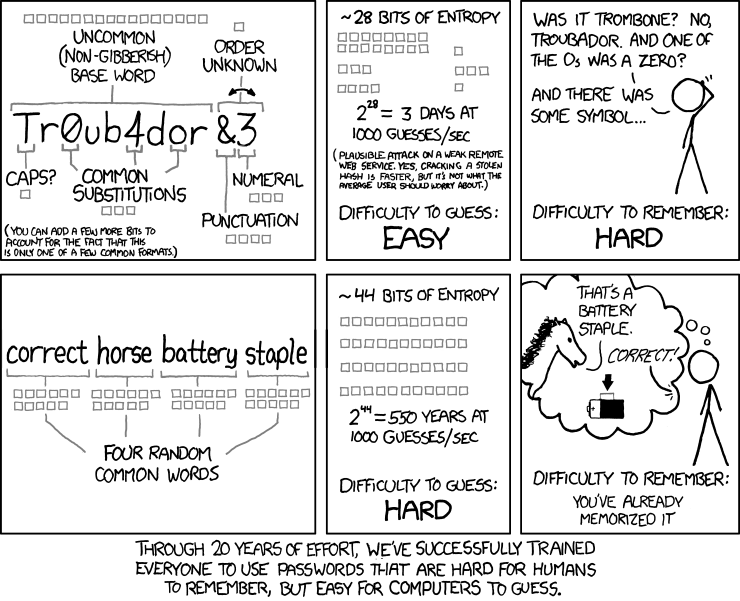
\includegraphics[width=\textwidth]{password_strength}
    \end{figure}
\end{frame}

\end{document}
